\begin{figure}[htbp]
\centering
\resizebox{\textwidth}{!}{%
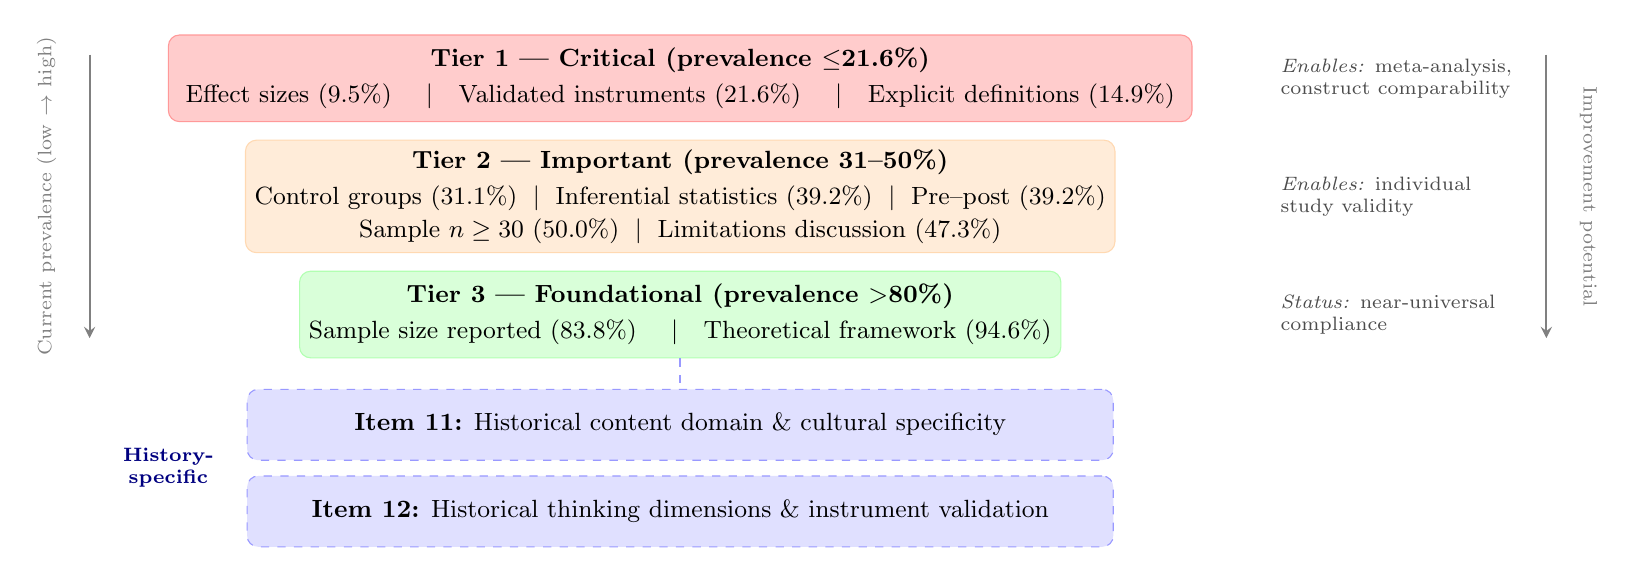
\begin{tikzpicture}[
    every node/.style={font=\small},
    tier/.style={
        rounded corners=4pt,
        minimum height=1.1cm,
        text=black,
        align=center,
        anchor=center,
    },
    histbox/.style={
        rounded corners=4pt,
        minimum height=0.9cm,
        text=black,
        align=center,
        anchor=center,
        fill=blue!12,
        draw=blue!40,
        dashed,
    },
    annot/.style={
        font=\scriptsize,
        text=black!70,
        anchor=west,
        align=left,
    },
]

% Vertical spacing
\def\yspacing{1.5}

% Tier widths (inverted pyramid: widest at top = highest priority)
\def\wA{13.0}   % Tier 1 (Critical)
\def\wB{11.0}   % Tier 2 (Important)
\def\wC{8.0}    % Tier 3 (Foundational)

% Annotation column
\def\rightcol{7.5}

% Y positions
\def\yA{0}
\pgfmathsetmacro{\yB}{\yA - \yspacing}
\pgfmathsetmacro{\yC}{\yB - \yspacing}
\pgfmathsetmacro{\yD}{\yC - 1.4}
\pgfmathsetmacro{\yE}{\yD - 1.1}

% --- Left margin arrow ---
\draw[-stealth, thick, black!50] (-7.5, \yA + 0.3) -- (-7.5, \yC - 0.3);
\node[rotate=90, anchor=south, font=\scriptsize, text=black!50] at (-7.8, {(\yA + \yC)/2})
    {Current prevalence (low $\rightarrow$ high)};

% --- Right margin arrow ---
\draw[-stealth, thick, black!50] (\rightcol + 3.5, \yA + 0.3) -- (\rightcol + 3.5, \yC - 0.3);
\node[rotate=-90, anchor=south, font=\scriptsize, text=black!50] at (\rightcol + 3.8, {(\yA + \yC)/2})
    {Improvement potential};

% --- Tier 1: Critical ---
\node[tier, fill=red!20, draw=red!40, minimum width=\wA cm] (T1) at (0, \yA)
    {\textbf{Tier~1 --- Critical (prevalence $\leq$21.6\%)}\\[2pt]
    Effect sizes (9.5\%) \quad\textbar\quad Validated instruments (21.6\%) \quad\textbar\quad Explicit definitions (14.9\%)};
\node[annot] at (\rightcol, \yA)
    {\textit{Enables:} meta-analysis,\\construct comparability};

% --- Tier 2: Important ---
\node[tier, fill=orange!15, draw=orange!30, minimum width=\wB cm] (T2) at (0, \yB)
    {\textbf{Tier~2 --- Important (prevalence 31--50\%)}\\[2pt]
    Control groups (31.1\%) \;\textbar\; Inferential statistics (39.2\%) \;\textbar\; Pre--post (39.2\%)\\[1pt]
    Sample $n \geq 30$ (50.0\%) \;\textbar\; Limitations discussion (47.3\%)};
\node[annot] at (\rightcol, \yB)
    {\textit{Enables:} individual\\study validity};

% --- Tier 3: Foundational ---
\node[tier, fill=green!15, draw=green!30, minimum width=\wC cm] (T3) at (0, \yC)
    {\textbf{Tier~3 --- Foundational (prevalence $>$80\%)}\\[2pt]
    Sample size reported (83.8\%) \quad\textbar\quad Theoretical framework (94.6\%)};
\node[annot] at (\rightcol, \yC)
    {\textit{Status:} near-universal\\compliance};

% --- History-specific additions ---
\node[histbox, minimum width=\wB cm] (H1) at (0, \yD)
    {\textbf{Item~11:} Historical content domain \& cultural specificity};
\node[histbox, minimum width=\wB cm] (H2) at (0, \yE)
    {\textbf{Item~12:} Historical thinking dimensions \& instrument validation};

% Label for history-specific items
\node[font=\scriptsize\bfseries, text=blue!50!black, anchor=east, align=center] at (-5.8, {(\yD + \yE)/2})
    {History-\\specific};

% Connecting lines from Tier 3 to history items
\draw[blue!40, dashed, thick] (T3.south) -- ++(0, -0.3) -| (H1.north);

\end{tikzpicture}%
}%
\caption{Priority tiers for the proposed reporting checklist, organised by current prevalence in the 74-study corpus (parenthetical percentages) and impact on evidence synthesis potential. Tier~1 items (red) have the lowest current prevalence but the highest impact: their adoption would enable meta-analytic synthesis and break the construct validity cascade at Stages~1 and~3 (Figure~\ref{fig:construct-validity-cascade}). Items~11--12 (blue) are history-education-specific additions addressing the disciplinary measurement deficit.}
\label{fig:checklist-priority-tiers}
\end{figure}
